\subsection{Impacts of the stabilizing force}
In setup 3 a and setup 4 each protein was stabilized with an external force acting on the FERM domain (see \autoref{motivation}). Therefore the dependency of the used observables is examined below.\\
\\
The force has a mean value of $1.47\,\forceunit$ and a standard deviation of $13.13\,\forceunit$. It is skewed to positive values. This is expected since positive values of the force require negative elongations $\Delta z$. If the connecting vector of F1 and F2 $\vec{d}_F$ is parallel to the z-axis, larger negative deviations require a stretching of $d_F$, which suppress these forces. \\
\\
Linear regressions show that none of the quantities $d_F$, $d_\text{F1-N}$, $d_\text{F2-C}$ and CA have a remarkable correlation to the applied force. Here remarkable means that either the regression result was not significant or that the obtained slope was so small, that a change of two standard deviations in force would not change the quantity noticeably.\\
\\
Also the distances between residue pairs are tested for correlation with the applied force. To this end, 10 different proteins without neighbours were picked out of the trajectories of setup 4, each for $1\,\si{\micro\second}$. On this dataset a linear regression was performed for each residue pair. \autoref{force:contactmap} shows the calculated Pearson correlation coefficient (only significant correlations with Pearson $\left|r\right| > 0.3$). The mean value of the slope for the positive correlated pair distances is $20.3\,\si{\pico\newton/\nano\metre}$ and $-19.7\,\si{\pico\newton/\nano\metre}$ for the negative correlated pair distances. Thus, the force can have large influences on these pairs. However, not all observed contacts at the interface (compare to \autoref{free:contact}) are effected.
%
%
%
\begin{figure}
	\centering
	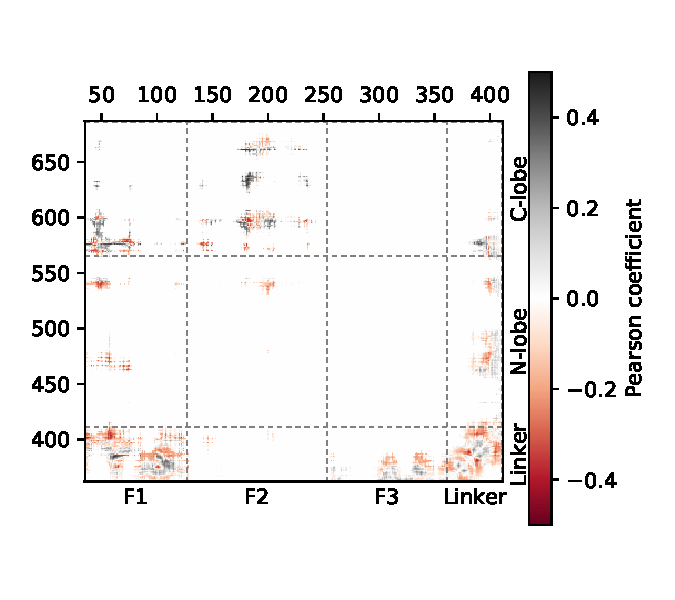
\includegraphics[width=.7\textwidth]{figures/results/interface_corr}
	\nicecaption{Correlations in contact map}{The contact map shows residue pairs, whose distance correlates with the applied force. The obtained slope is about $20\,\si{\pico\newton/\nano\metre}$.}
	\label{force:contactmap}
\end{figure}
%
%
%
\\
It is important to note that in this section only the observed quantities were tested for correlation with the force. It is however possible and probable, that due to this restriction, configurations or states are completely missing while others are over expressed. This effect can not be estimated, but should be kept in mind.